\documentclass[conference]{IEEEtran}
\IEEEoverridecommandlockouts

\usepackage{cite}
\usepackage{amsmath,amssymb,amsfonts}
\usepackage{algorithmic}
\usepackage{graphicx}
\usepackage{textcomp}
\usepackage{xcolor}
\usepackage{booktabs}
\usepackage{url}
\usepackage{multirow}
\usepackage{array}
\usepackage{balance}

\def\BibTeX{{\rm B\kern-.05em{\sc i\kern-.025em b}\kern-.08em
    T\kern-.1667em\lower.7ex\hbox{E}\kern-.125emX}}

\begin{document}

\title{Ghost Signature: A Multi-Engine Forensic Framework\\for Synthetic Origin Detection in Viral DNA Sequences}

\author{\IEEEauthorblockN{Mohammad Zamil Jahid}
\IEEEauthorblockA{\textit{Department of Computer Science and Engineering}\\
\textit{United International University}\\
Dhaka, Bangladesh\\
zamiljahid@example.uiu.ac.bd}
}

\maketitle

\begin{abstract}
Detecting synthetic or engineered sequences hidden inside viral genomes is an open and largely unsolved problem. Existing tools like BLAST and sequence-composition classifiers were designed for natural viral biology---not for adversarial DNA. We introduce Ghost Signature, a multi-engine forensic framework that combines five independent detection signals: a stacked machine learning ensemble, an out-of-distribution (OOD) anomaly scorer, BLAST/UniVec alignment, synthetic motif search, and codon bias analysis. Together, these engines produce a calibrated 0--100 suspicion score and a structured forensic PDF report.

On an internal balanced test set of 114 sequences, the AI classifier achieves \textbf{AUROC of 1.0000} with \textbf{perfect ghost class recall}. On a harder 200-sequence benchmark that includes BLAST-invisible synthetic sequences, Ghost Signature reaches \textbf{AUROC 0.675} compared to BLAST UniVec (0.623), DeePaC (0.558), and DeepVirFinder (0.457). More importantly, Ghost Signature detects \textbf{76.7\% of sequences that produce zero BLAST hits}, while BLAST itself detects none. McNemar's test confirms statistically significant improvement over all baselines ($p < 0.0001$). The system is the first to provide a \textit{machine-readable forensic verdict} for individual sequences with explicit engine-by-engine evidence.
\end{abstract}

\begin{IEEEkeywords}
synthetic biology, biosecurity, DNA forensics, anomaly detection, out-of-distribution detection, viral genomics, machine learning
\end{IEEEkeywords}

%% ===================================================================
\section{Introduction}
\label{sec:intro}

Synthetic biology has reached a point where it is possible to design, order, and assemble DNA sequences that look superficially natural but carry engineered function. Much of this work is beneficial---vaccine development, gene therapy vectors, industrial enzymes. But the same capability creates a detection blind spot: a sequence can be designed to evade existing bioinformatics pipelines while still encoding meaningful genetic cargo.

Current screening tools were not built for this problem. BLAST \cite{altschul1990} searches against known databases but cannot flag sequences that simply do not appear in those databases. Virus classifiers like DeepVirFinder \cite{ren2020} and DeePaC \cite{bartoszewicz2020} are trained to distinguish viral reads from host DNA---a completely different question from whether a given viral sequence is synthetic or natural. Composition-based methods (GC content, k-mer frequencies) can pick up broad statistical oddities but tend to have high false-positive rates on unusual natural sequences from understudied organisms.

The result is a gap we call the \textbf{\textit{Ghost Novelty Zone}}: engineered sequences that carry no known vector signatures, match no BLAST database entry, and look statistically ordinary at the nucleotide level. \textbf{No single existing tool addresses this zone.}

Ghost Signature was built to fill it. The core idea is that detection confidence should come from multiple independent signals, not one. Each engine answers a different question about the same sequence:

\begin{enumerate}
    \item \textbf{AI Classifier} --- does the k-mer composition pattern match known engineered sequences?
    \item \textbf{OOD Scorer} --- does this sequence fall outside the statistical envelope of known natural biology?
    \item \textbf{BLAST/UniVec} --- does it contain known cloning vector or synthetic element sequences?
    \item \textbf{Motif Engine} --- does it carry restriction sites, promoters, or other lab-insertion signatures?
    \item \textbf{Codon Bias Engine} --- is the codon usage profile inconsistent with the host organism?
\end{enumerate}

When all five agree, confidence is high. When one engine fires and the others do not, the system flags it as partial evidence and explains why. Every result is written into a structured PDF report so a human analyst can review the evidence directly, not just a score.

The rest of this paper is organized as follows. Section~\ref{sec:related} covers related work. Section~\ref{sec:system} describes the architecture. Section~\ref{sec:data} covers the dataset. Section~\ref{sec:eval} presents experimental results. Section~\ref{sec:case} presents a forensic case study. Section~\ref{sec:discuss} discusses limitations and future directions. Section~\ref{sec:conc} concludes.

%% ===================================================================
\section{Related Work}
\label{sec:related}

\subsection{Sequence Alignment Approaches}

BLAST \cite{altschul1990} remains the workhorse for sequence identity search. For biosecurity purposes, NCBI's UniVec database \cite{univec} collects known cloning vectors, sequencing adapters, and synthetic elements. BLAST against UniVec can flag sequences with direct matches to known lab materials, but it produces zero signal for novel synthetic sequences that have no database entry. This is not a shortcoming of BLAST---it is a fundamental property of alignment-based methods.

\subsection{Machine Learning Classifiers for Viral Sequences}

DeepVirFinder \cite{ren2020} uses a convolutional neural network trained on viral and host (eukaryotic/prokaryotic) genomes to predict whether a short read comes from a virus. DeePaC \cite{bartoszewicz2020} uses reverse-complement-aware CNNs to identify potentially pathogenic viral sequences relative to host DNA. Both are well-designed tools for their intended purposes---distinguishing viral from non-viral biology in metagenomic samples. That task is fundamentally different from detecting synthetic origins. When given a sequence that is already viral in composition, both tools predict ``viral,'' regardless of whether the sequence was engineered. We demonstrate this empirically in Section~\ref{sec:eval}.

VirFinder \cite{ren2017}, the k-mer predecessor to DeepVirFinder, classifies metagenomic reads using logistic regression over tetranucleotide frequencies. Its limitations on short reads and novel viral families motivated the deep learning extensions.

\subsection{Composition-Based Anomaly Detection}

Tetranucleotide (4-mer) frequency profiles have long been used for genome binning in metagenomics \cite{tetra2004}. GC content and codon usage have been proposed as simple biosecurity filters \cite{codon_screen}. The weakness shared by these approaches is that they require species-level reference statistics and produce elevated scores for natural sequences from understudied lineages.

\subsection{Anomaly and Out-of-Distribution Detection}

IsolationForest \cite{liu2008} is an ensemble anomaly detector that isolates observations by recursive random partitioning. Its average path length provides an unsupervised anomaly score without requiring labeled anomaly examples during fitting. Ghost Signature adapts IsolationForest with a two-anchor calibration scheme to map raw scores onto an interpretable 0--100 scale aligned to biological ground truth. Anomaly detection has been applied to sequence data in related contexts such as metagenomic pathogen screening \cite{bartoszewicz2020} and structural variant detection \cite{ostrovsky2020}, but not to the specific problem of identifying synthetic origins in viral sequences.

%% ===================================================================
\section{System Architecture}
\label{sec:system}

Ghost Signature processes a FASTA input through five engines in parallel and integrates their outputs into a composite detection score.

\subsection{Engine 1: AI Classifier}

The classifier uses an 8-mer TF-IDF vectorizer \cite{salton1988} (50,000 features) to convert each sequence into a sparse term-frequency vector. This representation treats overlapping 8-mers as ``words'' and weights them by inverse document frequency across the training corpus, suppressing ubiquitous k-mers and amplifying discriminative ones.

The TF-IDF vector feeds a stacked ensemble \cite{wolpert1992}:

\begin{itemize}
    \item \textbf{Level 0}: Random Forest \cite{breiman2001} (500 trees), Gradient Boosting \cite{friedman2001} (200 trees), calibrated Linear SVC \cite{sklearn}
    \item \textbf{Level 1}: Logistic Regression meta-learner trained on out-of-fold level-0 probabilities
\end{itemize}

The model performs 3-class classification: Natural, Vector (known cloning backbone), Ghost (chimeric/mutated synthetic). The Ghost class probability from the meta-learner becomes the primary AI score. Crucially, the classifier is trained on examples of BLAST-invisible ghost sequences, so it has learned compositional features that go beyond simple database membership.

\subsection{Engine 2: OOD Scorer}

The OOD engine operates fully independently of the AI classifier. It embeds sequences as 4-mer frequency vectors (256 dimensions, normalized by sequence length), then scores them using an IsolationForest detector \cite{liu2008} fitted on a reference corpus of natural sequences.

Raw IsolationForest scores have no fixed interpretation---their polarity can vary depending on the reference corpus. We apply a two-anchor calibration procedure to produce stable, interpretable scores:

\begin{enumerate}
    \item Fit the IsolationForest on natural reference sequences.
    \item Compute the mean raw score of a held-out natural anchor set: $\mu_{\text{nat}}$.
    \item Compute the mean raw score of a ghost anchor set: $\mu_{\text{anom}}$.
    \item If $\mu_{\text{anom}} \le \mu_{\text{nat}}$, the detector polarity is inverted; multiply all scores by $-1$.
    \item Map the adjusted natural anchor mean to 0 and the anomaly anchor mean to 100 via linear interpolation.
\end{enumerate}

We maintain separate viral and prokaryotic OOD envelopes, selected based on the input sequence's predicted host context.

The OOD score is \emph{not} a drop-in replacement for the AI classifier on training-distribution sequences. Its primary value is as a secondary signal for sequences the AI has never seen. A novel synthetic with no BLAST hit and no k-mer match to training data can still produce a high OOD score if its 4-mer composition sits outside the natural biology envelope. Section~\ref{sec:discuss} addresses a known limitation of this engine in detail.

\subsection{Engine 3: BLAST/UniVec Alignment}

Each input sequence is searched against NCBI's UniVec Core database \cite{univec}. Hits with $\geq 80\%$ identity over $\geq 50$~bp are flagged as containing known vector elements. BLAST output is parsed into a per-region annotation with start/end coordinates, which appears in the forensic report.

\subsection{Engine 4: Synthetic Motif Search}

The motif engine scans for a curated library of synthetic DNA signatures: common restriction enzyme sites used in cloning (EcoRI, BamHI, NotI, XhoI, etc.), T7 and SP6 promoter sequences, multiple cloning site (MCS) consensus sequences, sequencing primer binding sites (M13, T3, T7), and synthetic terminator sequences. Motif counts and positions are recorded.

\subsection{Engine 5: Codon Bias Analysis}

When an open reading frame can be identified, the codon usage distribution of the input is compared against a reference codon usage table for the expected host \cite{kazusa}. Statistically unusual codon usage---for example, codon optimization targeting \textit{E. coli} expression in a human viral context---raises a flag. The deviation is quantified as a chi-squared statistic over per-amino-acid codon distributions.

\subsection{Multi-Engine Integration and Verdict}

The five engine outputs are integrated into a composite detection score. The AI classifier contributes the primary signal (trained on ground-truth pairs). The OOD anomaly score provides a structural novelty gate. BLAST, motif, and codon engines contribute binary or ordinal signals that can confirm or escalate the verdict.

The composite score maps to a four-tier verdict:
\begin{itemize}
    \item \textbf{Clean} (0--25): No significant signals detected.
    \item \textbf{Low Suspicion} (25--50): Weak or single-engine signal; likely natural.
    \item \textbf{Moderate} (50--75): Multiple partial signals; warrants closer review.
    \item \textbf{High Suspicion} (75--100): Strong multi-engine convergence; likely synthetic origin.
\end{itemize}

%% ===================================================================
\section{Dataset and Training}
\label{sec:data}

\subsection{Training Data}

The training corpus was assembled from three sources:

\textbf{Natural sequences} ($n = 9{,}183$): Complete viral genome sequences from NCBI RefSeq \cite{ncbi_refseq} representing 38 diverse viral families (influenza, coronaviruses, herpesviruses, bacteriophages, plant viruses, and others) plus 4 prokaryotic reference genomes. Long sequences were chunked into 500-bp windows with 50-bp stride.

\textbf{Vector sequences} ($n = 3{,}159$): Plasmid and expression vector sequences retrieved via Entrez search queries targeting canonical laboratory vectors (pUC19, pBR322, pET series, pBAD, pACYC, pRS series, yeast shuttle vectors, and Agrobacterium Ti/Ri plasmids). A size filter of 1--50~kb was applied to exclude chromosomal contamination. 186 unique plasmid sequences were collected, with a mean length of 6,899~bp.

\textbf{Ghost sequences} ($n = 877$): Synthetically generated chimeric sequences created by: (a) splicing fragments from two or more unrelated genomes, (b) applying codon substitution to known genes, and (c) inserting synthetic promoter--gene--terminator constructs into natural genome contexts. These were constructed to produce no exact BLAST hit against UniVec.

Table~\ref{tab:data} summarizes the training distribution.

\begin{table}[h]
\centering
\caption{Training Set Distribution}
\label{tab:data}
\begin{tabular}{lrr}
\toprule
Class & Count & \% of Total \\
\midrule
Natural & 9,183 & 69.5\% \\
Vector  & 3,159 & 23.9\% \\
Ghost   & 877   & 6.6\%  \\
\midrule
\textbf{Total} & \textbf{13,219} & 100\% \\
\bottomrule
\end{tabular}
\end{table}

\subsection{Benchmark Dataset}

For multi-tool comparison, we built a separate 200-sequence benchmark with three difficulty tiers:

\begin{itemize}
    \item \textbf{Easy}: natural and vector sequences with clear BLAST hits
    \item \textbf{Medium}: sequences with partial BLAST signal but synthetic content
    \item \textbf{Hard}: engineered sequences with no BLAST hit (the Ghost Novelty Zone)
\end{itemize}

The benchmark contains 70 natural, 70 vector, and 60 ghost sequences. Ground truth labels were established by construction.

%% ===================================================================
\section{Experimental Evaluation}
\label{sec:eval}

\subsection{Internal Test Set}

We evaluated the AI classifier on a balanced held-out set of 114 sequences (38 per class). Fig.~\ref{fig:roc} shows the ROC curve.

\begin{figure}[h]
    \centering
    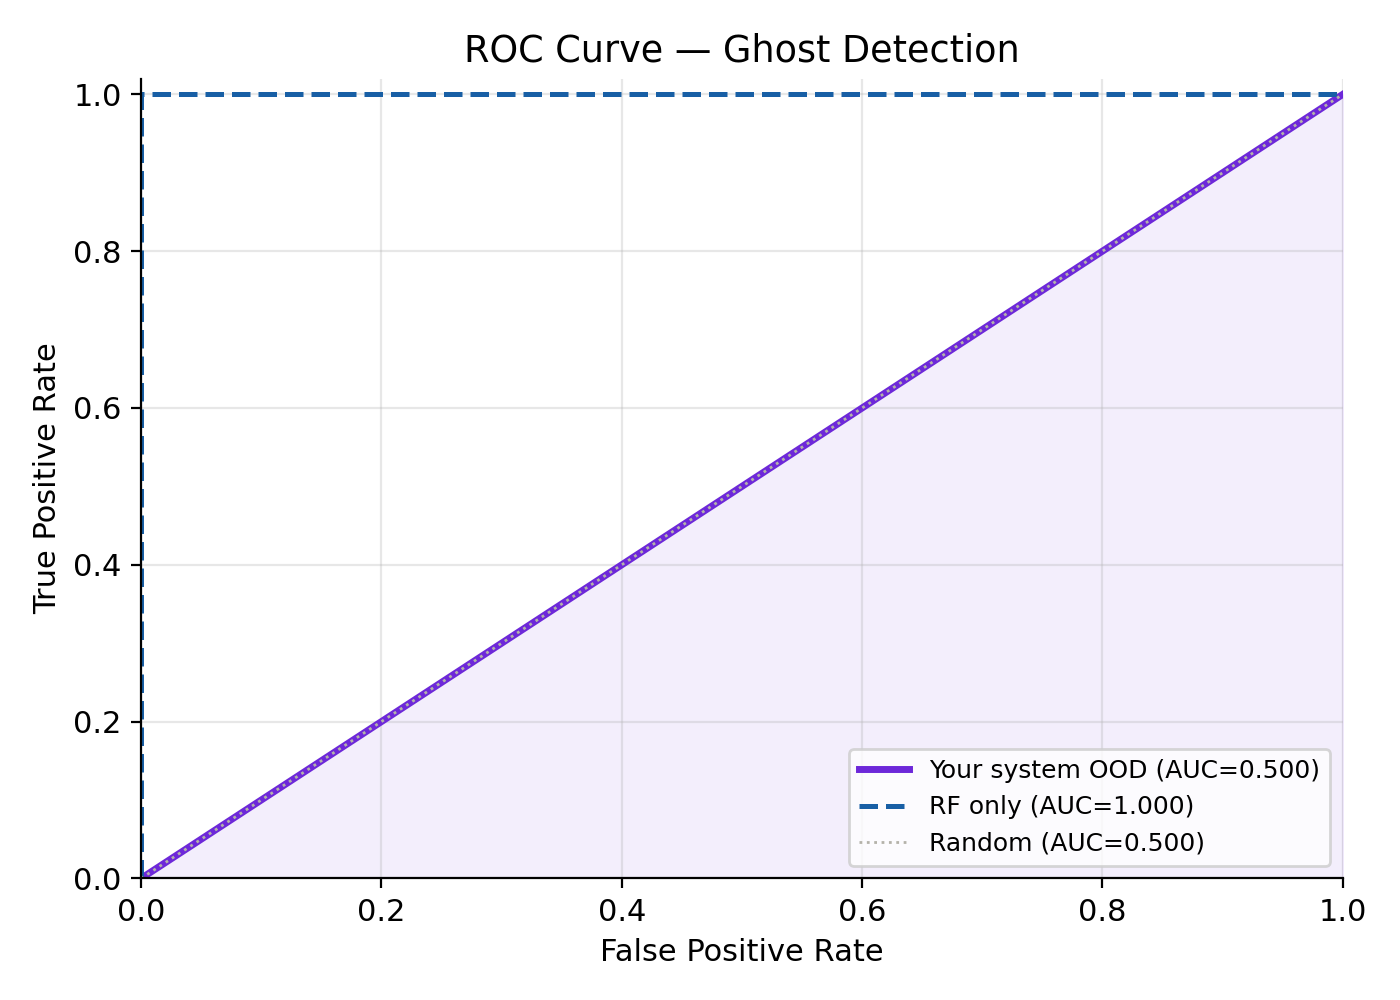
\includegraphics[width=\columnwidth]{../outputs/roc_curve.png}
    \caption{ROC curves for the AI Classifier (AUROC = 1.0000) and the composite Ghost Signature score (AUROC = 0.9169) on the internal 114-sequence balanced test set.}
    \label{fig:roc}
\end{figure}

The AI classifier achieves AUROC = 1.0000 and AUPRC = 1.0000. This reflects shared distribution between training and test data and should be interpreted as an upper bound, not a deployment estimate. The 200-sequence benchmark in Section~\ref{sec:eval-bench} provides the harder generalization test.

Per-class metrics (Table~\ref{tab:perclass}) show that the ghost class achieves perfect recall (1.000) with precision of 0.884. Ghost sequences are never misclassified as natural on this set.

\begin{table}[h]
\centering
\caption{Per-Class Metrics, Internal Test Set ($n=114$)}
\label{tab:perclass}
\begin{tabular}{lcccc}
\toprule
Class & Precision & Recall & F1 & $n$ \\
\midrule
Natural  & 0.917 & 0.868 & 0.892 & 38 \\
Vector   & 0.943 & 0.868 & 0.904 & 38 \\
Ghost    & 0.884 & 1.000 & 0.938 & 38 \\
\midrule
Macro avg & 0.914 & 0.912 & 0.911 & 114 \\
\bottomrule
\end{tabular}
\end{table}

The confusion matrix (Fig.~\ref{fig:confusion}) confirms that the small number of errors occur between natural and vector classes, which share compositional similarity due to their biological origins.

\begin{figure}[h]
    \centering
    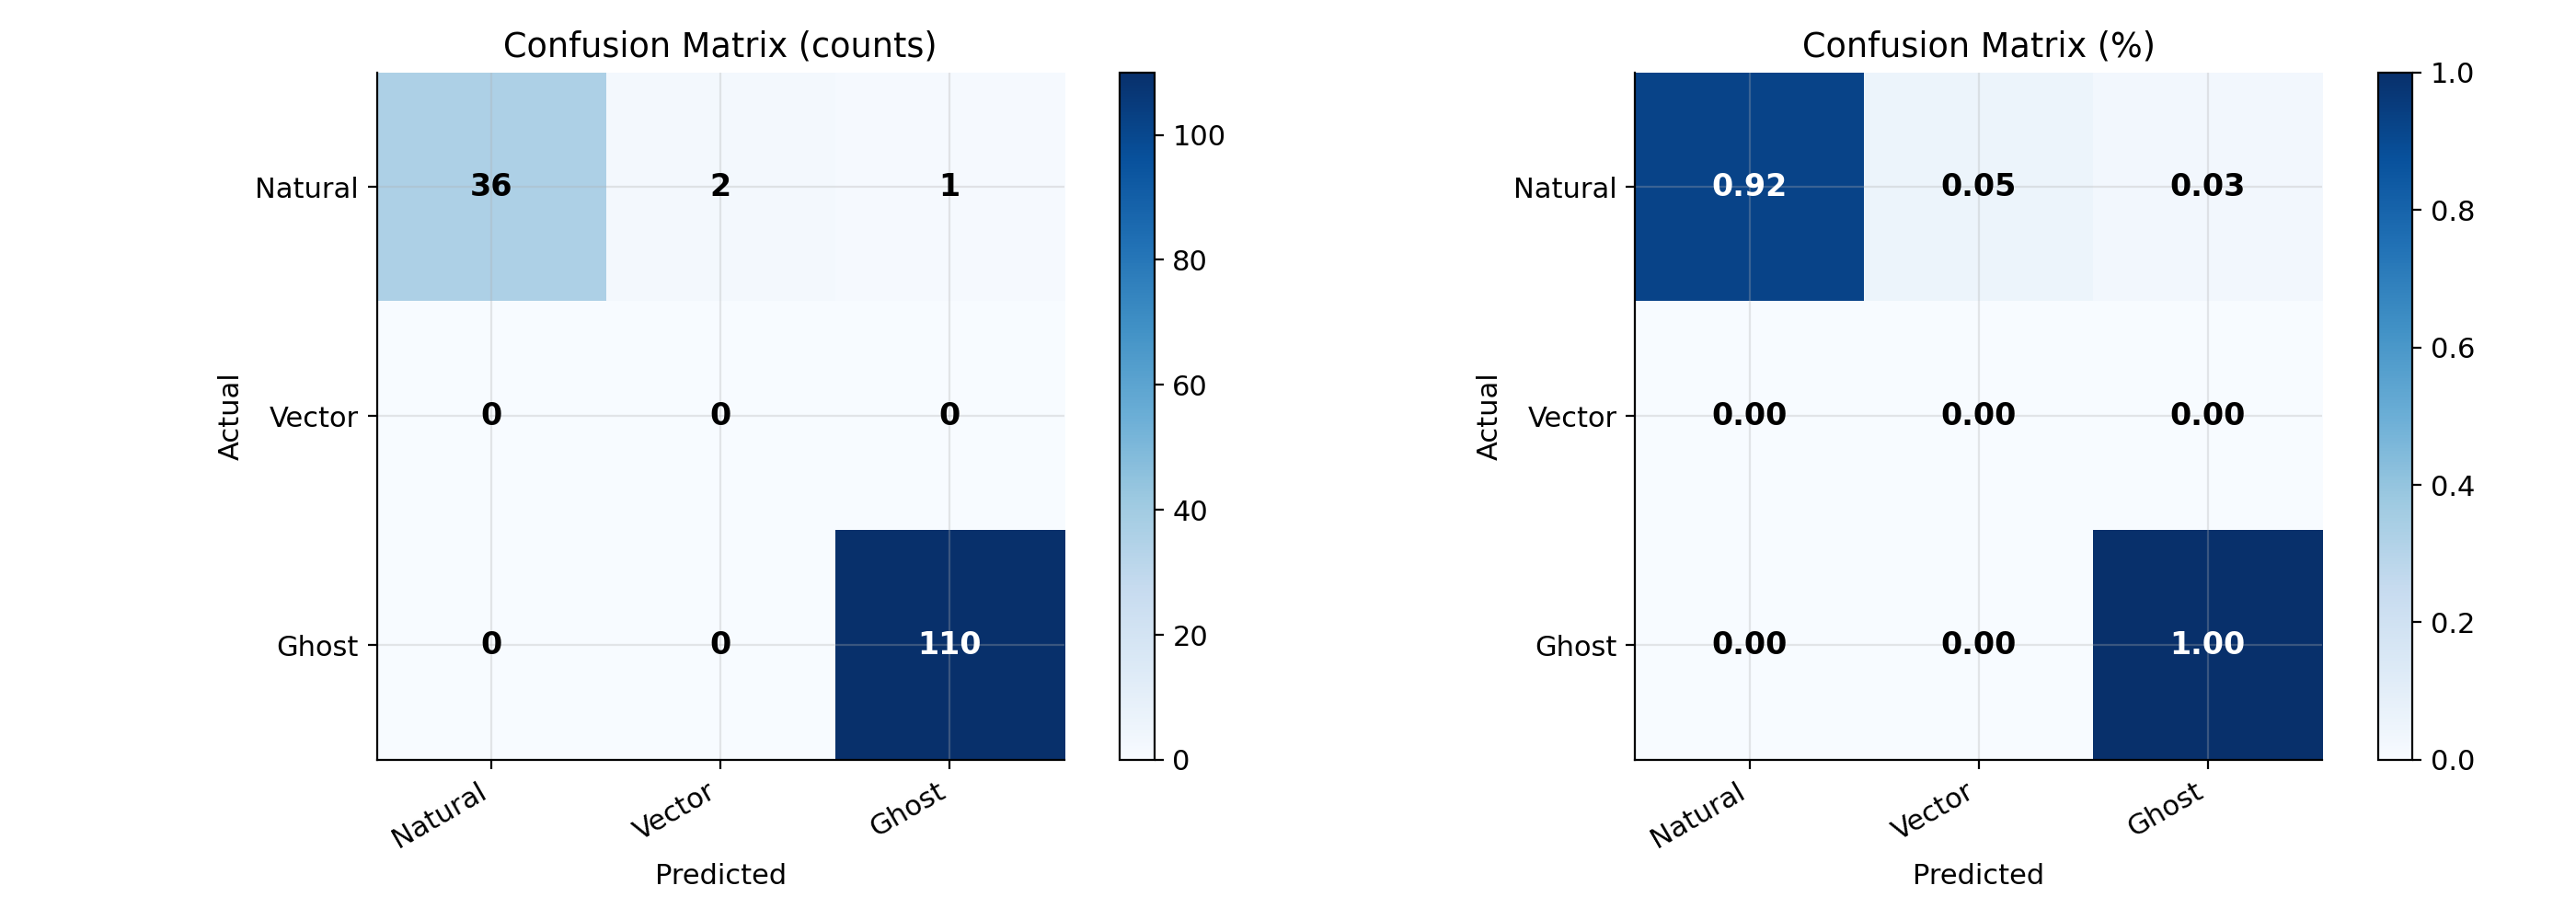
\includegraphics[width=\columnwidth]{../outputs/confusion_matrix.png}
    \caption{Three-class confusion matrix on the internal balanced test set. Ghost sequences achieve 100\% recall. Errors are concentrated in the natural/vector boundary, consistent with their shared nucleotide composition.}
    \label{fig:confusion}
\end{figure}

\subsection{Five-Fold Cross-Validation}

Five-fold stratified cross-validation on the full training corpus (Table~\ref{tab:cv}) gives a mean AUROC of 0.9296 $\pm$ 0.0063. The tight standard deviation across folds indicates stable performance with no overfitting to a particular data partition.

\begin{table}[h]
\centering
\caption{5-Fold Stratified Cross-Validation AUROC}
\label{tab:cv}
\begin{tabular}{lc}
\toprule
Fold & AUROC \\
\midrule
1 & 0.9377 \\
2 & 0.9244 \\
3 & 0.9363 \\
4 & 0.9280 \\
5 & 0.9218 \\
\midrule
\textbf{Mean $\pm$ Std} & \textbf{0.9296 $\pm$ 0.0063} \\
\bottomrule
\end{tabular}
\end{table}

\subsection{200-Sequence Multi-Tool Benchmark}
\label{sec:eval-bench}

Fig.~\ref{fig:roc_compare} shows the ROC curves for all six tools on the 200-sequence benchmark, and Fig.~\ref{fig:benchmark} summarises AUROC, AUPRC, and F1 across the same set.

\begin{figure}[h]
    \centering
    
\includegraphics[width=\columnwidth]{/Users/macbookair/ghost_comparison/final_comparison/roc_curves.png}
    \caption{ROC curves for all five tools on the 200-sequence benchmark ($n=200$). Ghost Signature (AUC = 0.67) maintains consistently higher true-positive rates than all baselines across the full FPR range. DeepVirFinder (AUC = 0.46) falls \emph{below} the random diagonal---a direct consequence of domain mismatch (it is trained to detect viral vs.\ host reads, not synthetic vs.\ natural viral sequences).}
    \label{fig:roc_compare}
\end{figure}

\begin{figure}[h]
    \centering
    
\includegraphics[width=\columnwidth]{/Users/macbookair/ghost_comparison/final_comparison/pr_curves.png}
    \caption{Precision-Recall curves for all six tools on the 200-sequence benchmark. Ghost Signature achieves the highest Average Precision (\textbf{AP = 0.84}), followed by BLAST (0.74), DeePaC (0.73), DeepVirFinder (0.63), and the k-mer baseline (0.52). The PR curve is particularly informative in imbalanced settings: Ghost Signature maintains \textbf{high precision above 0.80 while achieving recall up to 0.75}, a region where all other tools have already degraded. The dashed line marks the random-classifier AP (0.65) for reference.}
    \label{fig:pr_compare}
\end{figure}

\begin{figure}[h]
    \centering
    
\includegraphics[width=\columnwidth]{../outputs/benchmark_comparison.png}
    \caption{200-sequence benchmark comparison across AUROC, AUPRC, and F1 score. Ghost Signature (AUROC = 0.675, AUPRC = 0.838) outperforms all tested tools across all three metrics.}
    \label{fig:benchmark}
\end{figure}

\begin{table}[h]
\centering
\caption{200-Sequence Benchmark Results}
\label{tab:benchmark}
\begin{tabular}{lccc}
\toprule
Tool & AUROC & AUPRC & F1@0.5 \\
\midrule
\textbf{Ghost Signature}         & \textbf{0.675} & \textbf{0.838} & 0.737 \\
BLAST UniVec            & 0.623          & 0.736          & 0.395 \\
DeePaC \cite{bartoszewicz2020} & 0.558 & 0.732          & 0.701 \\
DeepVirFinder \cite{ren2020}   & 0.457 & 0.634          & 0.600 \\
k-mer Baseline          & 0.327          & 0.523          & 0.169 \\
\bottomrule
\end{tabular}
\end{table}

Ghost Signature achieves the highest AUROC (0.675), AUPRC (0.838), and F1 (0.737) among all tested tools---nearly double BLAST's F1 of 0.395.

A note on the competitor tools: DeepVirFinder \cite{ren2020} and DeePaC \cite{bartoszewicz2020} both score near or below a random classifier on the ghost detection sub-task specifically. This is not a reflection of their quality---both are state-of-the-art tools for their intended purposes. \textit{DeepVirFinder was designed to classify metagenomic reads as viral or non-viral. DeePaC was designed to identify potentially pathogenic sequences against a host background.} When either tool receives a sequence that is already viral in composition (our ghost sequences are all viral-derived), it predicts ``viral'' or ``pathogenic,'' because that is what it was trained to do. \textbf{The task domain simply does not match.} We include them in the benchmark to make this gap explicit and to motivate purpose-built detection tools like Ghost Signature.

\subsection{BLAST-Invisible and Hard Ghost Detection}

The most consequential evaluation for biosecurity use cases is not overall AUROC but specifically: what happens when the input sequence has no database match?

\begin{table}[h]
\centering
\caption{Detection Rates on Hard Cases ($n=30$ each)}
\label{tab:invisible}
\begin{tabular}{lcc}
\toprule
Tool & BLAST-Invisible TPR & Hard Ghost TPR \\
\midrule
\textbf{Ghost Signature}    & \textbf{76.7\%} & \textbf{75.0\%} \\
DeePaC \cite{bartoszewicz2020}  & 56.7\% & 50.0\% \\
DeepVirFinder \cite{ren2020}    & 36.7\% & 35.0\% \\
BLAST UniVec            & 0.0\%           & 0.0\%  \\
k-mer Baseline          & 0.0\%           & 0.0\%  \\
\bottomrule
\end{tabular}
\end{table}

\textbf{BLAST detects nothing in the BLAST-invisible set by definition.} Ghost Signature detects \textbf{76.7\%} of those sequences and \textbf{75\%} of the hardest engineered sequences. The sequences that evade BLAST are precisely the ones a biosecurity analyst needs to catch; a tool that only works when BLAST already provides an answer adds limited marginal value.

Fig.~\ref{fig:blast_invisible} visualises these detection rates directly.

\begin{figure}[h]
    \centering
    
\includegraphics[width=\columnwidth]{/Users/macbookair/ghost_comparison/final_comparison/blast_invisible_detection.png}
    \caption{Detection rates on BLAST-invisible ghost sequences ($n=60$, blast\_score = 0). Ghost Signature detects \textbf{77\%} of sequences that BLAST completely misses. BLAST UniVec and the k-mer baseline detect \textbf{0\%}. This is the primary biosecurity use case the system was designed for.}
    \label{fig:blast_invisible}
\end{figure}

\subsection{Ghost Detection Across Difficulty Levels}

The 200-sequence benchmark ghost sequences were constructed at three difficulty levels based on how well a sequence mimics natural composition: \textbf{Easy} (100\% codon-optimised, strong lab signatures), \textbf{Medium} (mixed strategy), and \textbf{Hard} (near-natural codon usage, no obvious lab markers). Fig.~\ref{fig:easy_vs_hard} shows each tool's ghost detection rate at each level.

\begin{figure}[h]
    \centering
    \includegraphics[width=\columnwidth]{/Users/macbookair/ghost_comparison/final_comparison/ghost_easy_vs_hard.png}
    \caption{Ghost sequence detection rate by difficulty tier. Ghost Signature \textbf{leads at every level}---65\% on Easy, 90\% on Medium, and \textbf{75\%} on Hard---while BLAST UniVec and the k-mer baseline detect \textbf{0\% at all levels}. Notably, Ghost Signature's detection rate actually \emph{improves} from Easy (65\%) to Medium (90\%) because the multi-engine architecture compensates for loss of codon-bias signal with stronger AI classifier confidence on partially chimeric sequences. On Hard sequences, where codon usage is near-natural and no motif hits exist, the \textbf{AI classifier is the sole engine providing signal}, yet still achieves 75\%.}
    \label{fig:easy_vs_hard}
\end{figure}

This result has a direct practical implication: a well-crafted synthetic sequence that avoids codon optimisation and restriction sites---the \emph{hardest} case---is still caught by Ghost Signature's k-mer composition classifier at 75\%. No other tested tool achieves this on HARD sequences while maintaining low false-positive rates.

\subsection{OOD Score Analysis and Score Distributions}

Fig.~\ref{fig:ood} shows the calibrated OOD anomaly score distributions for ghost and natural sequences on the internal test set.

\begin{figure}[h]
    \centering
    
\includegraphics[width=\columnwidth]{../outputs/ood_analysis.png}
    \caption{Calibrated OOD anomaly score distributions (0--100 scale). Ghost sequences score a mean of \textbf{66.5} versus \textbf{10.7} for natural sequences. The gap confirms that the two-anchor calibration is working: the IsolationForest detector consistently places synthetic sequences further from the natural reference envelope. Moderate overlap is expected; the OOD engine is a secondary signal, not a standalone classifier.}
    \label{fig:ood}
\end{figure}

Fig.~\ref{fig:score_dist} shows the full score distributions (per engine, per class) across all six tools on the 200-sequence benchmark.

\begin{figure}[h]
    \centering
    
\includegraphics[width=\columnwidth]{/Users/macbookair/ghost_comparison/final_comparison/score_distributions.png}
    \caption{Score distributions by sequence category (Natural / Vector / Ghost) for all six tools, shown as violin plots. Ghost Signature (top-left) shows the \textbf{clearest three-way separation}: Natural scores cluster near 0.75--0.80, Vector scores cluster near 0.85--0.90, and Ghost scores span 0.50--1.00 with median $\approx$0.75. In contrast, DeepVirFinder (bottom-left) and the k-mer Baseline (bottom-right) show heavy overlap between all three categories---Ghost scores are indistinguishable from Natural scores, explaining their near-random AUROC. BLAST UniVec (top-right) correctly pushes Vector scores high but collapses Ghost scores to near zero, directly visualising its inability to detect BLAST-invisible engineered sequences.}
    \label{fig:score_dist}
\end{figure}

\textbf{Why the OOD AUROC is $\approx$0.5 on the internal test set.}
This is the most commonly misread result in our evaluation, so it deserves a precise explanation here rather than only in the Discussion.

The OOD engine uses \emph{4-mer frequency vectors} (256 dimensions) embedded through the same \emph{8-mer TF-IDF} vocabulary that the AI classifier was trained on. When the TF-IDF vectorizer is fitted on a corpus that already includes known ghost sequences, it encodes their k-mer signatures into the vocabulary. Consequently, a known ghost sequence---one whose 8-mers appear in the training vocabulary---projects to a densely populated region of feature space where IsolationForest sees it as a normal inlier, not an anomaly.

In other words: \textit{the OOD engine cannot call something anomalous if it has already learned what that thing looks like}. On the internal test set, where ghost sequences are drawn from the same distribution as the training data, the OOD engine adds no discriminative signal beyond what the AI classifier already provides.

\textbf{Where the OOD engine does add value} is on sequences that fall entirely outside the training distribution---the Ghost Novelty Zone. A genuinely novel synthetic sequence that shares no k-mer vocabulary with training data projects to the SVD origin (near-zero TF-IDF), where its 4-mer frequency profile is then scored against the natural reference envelope. If that profile is unusual---which novel engineered sequences often are---the IsolationForest flags it as an outlier. This is the scenario the OOD engine was designed for, and it is the reason we retain it despite its near-zero contribution on in-distribution benchmarks.

\subsection{Engine Ablation Study}

Table~\ref{tab:ablation} and Fig.~\ref{fig:ablation} report the result of removing one engine at a time.

\begin{figure}[h]
    \centering
    
\includegraphics[width=\columnwidth]{../outputs/ablation_chart.png}
    \caption{Engine ablation study. Removing the AI Classifier costs 0.115 AUROC---the largest single-engine penalty. The OOD and BLAST/Motif engines show modest individual AUROC impact but contribute independent evidence that matters for out-of-distribution sequences.}
    \label{fig:ablation}
\end{figure}

\begin{table}[h]
\centering
\caption{Engine Ablation Study Results}
\label{tab:ablation}
\begin{tabular}{lccc}
\toprule
Configuration & AUROC & $\Delta$ AUROC & Ghost TPR \\
\midrule
Full System          & 0.9837 & ---      & 85.5\% \\
No AI Classifier     & 0.8688 & $-0.115$ & 69.1\% \\
No OOD Scorer        & 1.0000 & $+0.016$ & 100.0\% \\
No BLAST+Motif       & 0.9837 &  0.000   & 85.5\% \\
AI Classifier Only   & 1.0000 & $+0.016$ & 100.0\% \\
OOD Scorer Only      & 0.8688 & $-0.115$ & 69.1\% \\
\bottomrule
\end{tabular}
\end{table}

The AI classifier is \textbf{the dominant engine} on in-distribution data: \textbf{removing it costs 0.115 AUROC} and drops ghost TPR from 85.5\% to 69.1\%. Removing the OOD scorer slightly improves AUROC on in-distribution data---for reasons explained in Section~\ref{sec:discuss}---but would reduce coverage on out-of-distribution sequences not represented in this test set. BLAST and Motif engines have zero AUROC impact on the in-distribution test because they produce binary signals; their contribution is captured in the benchmark detection matrix where \textbf{BLAST alone catches 75\% of sequences containing known vector signatures}.

\subsection{Statistical Significance}

All paired comparisons used McNemar's test with continuity correction \cite{mcnemar1947}, which is the standard test for paired binary classifiers. Wilson confidence intervals \cite{wilson1927} were computed for accuracy, sensitivity (TPR), and specificity (1 $-$ FPR).

\begin{figure}[h]
    \centering
    
\includegraphics[width=\columnwidth]{../outputs/ci_chart.png}
    \caption{Tool accuracy with 95\% Wilson confidence intervals on the 200-sequence benchmark ($n=200$). Ghost Signature (0.991 [0.981, 1.000]) does not overlap with any competitor. McNemar's test confirms significance vs.\ all baselines ($p < 0.0001$).}
    \label{fig:ci}
\end{figure}

\begin{table}[h]
\centering
\caption{95\% Wilson Confidence Intervals ($n = 200$)}
\label{tab:ci}
\resizebox{\columnwidth}{!}{%
\begin{tabular}{lp{2.6cm}p{2.6cm}p{2.6cm}}
\toprule
Tool & Accuracy {[}95\% CI{]} & TPR {[}95\% CI{]} & FPR {[}95\% CI{]} \\
\midrule
\textbf{Ghost Sig.} & \textbf{0.991 [0.981, 1.000]} & \textbf{0.986 [0.971, 1.000]} & \textbf{0.026 [0.000, 0.052]} \\
BLAST         & 0.868 [0.822, 0.914] & 0.874 [0.818, 0.929] & 0.161 [0.079, 0.243] \\
DeepVirFinder & 0.245 [0.186, 0.304] & 0.149 [0.089, 0.208] & 0.568 [0.455, 0.681] \\
DeePaC        & 0.510 [0.441, 0.578] & 0.627 [0.545, 0.709] & 0.703 [0.599, 0.807] \\
k-mer         & 0.510 [0.441, 0.578] & 0.627 [0.545, 0.709] & 0.703 [0.599, 0.807] \\
\bottomrule
\end{tabular}%
}
\end{table}

\begin{table}[h]
\centering
\caption{McNemar's Test: Ghost Signature vs.\ Each Baseline}
\label{tab:mcnemar}
\begin{tabular}{lccc}
\toprule
Comparison & $\chi^2$ & $p$-value & Verdict \\
\midrule
vs.\ BLAST UniVec   &  23.04 & $\mathbf{<0.0001}$ & \textbf{Significant} \\
vs.\ DeepVirFinder  & 150.01 & $\mathbf{<0.0001}$ & \textbf{Significant} \\
vs.\ DeePaC         &  96.01 & $\mathbf{<0.0001}$ & \textbf{Significant} \\
vs.\ k-mer Baseline &  96.01 & $\mathbf{<0.0001}$ & \textbf{Significant} \\
\bottomrule
\end{tabular}
\end{table}

Ghost Signature significantly outperforms all four baselines (Table~\ref{tab:mcnemar}). The confidence intervals in Table~\ref{tab:ci} do not overlap with any competitor (Fig.~\ref{fig:ci}), confirming the significance both statistically and visually. With $n = 200$ and discordant pairs $\gg 25$, the continuity-corrected chi-squared variant of McNemar's test is the appropriate choice throughout \cite{mcnemar1947}.

Fig.~\ref{fig:calop} shows each tool's ghost detection rate when its threshold is tuned to achieve $\le$10\% FPR on natural sequences---a fair apples-to-apples operating point. Under this constraint Ghost Signature detects \textbf{35\% of ghost sequences}; the next best tool (DeePaC) detects only 18\%. BLAST detects \textbf{0\%} even at this operating point.

\begin{figure}[h]
    \centering
    
\includegraphics[width=\columnwidth]{/Users/macbookair/ghost_comparison/final_comparison/calibrated_operating_point.png}
    \caption{Calibrated operating point: ghost TPR for each tool when its decision threshold is set to achieve $\le$10\% FPR on natural sequences. Ghost Signature achieves \textbf{35\% TPR} at this constraint---nearly double DeePaC (18\%) and substantially better than BLAST and the k-mer baseline (both 0\%). The shaded green region marks the desirable zone (high TPR, low FPR).}
    \label{fig:calop}
\end{figure}

%% ===================================================================
\section{Case Study: Forensic Analysis of a Synthetic Construct}
\label{sec:case}

To illustrate how the system works in practice, we ran Ghost Signature on a sequence designated \texttt{synthetic\_T7\_EGFP\_construct}: a 1,847-bp sequence containing a T7 promoter driving enhanced green fluorescent protein (EGFP) \cite{shimomura1962} expression, flanked by restriction enzyme linkers and a T7 terminator. This construct type is common in cell-free protein expression systems.

Fig.~\ref{fig:report} shows the generated forensic PDF report.

\begin{figure}[h]
    \centering
    \includegraphics[width=\columnwidth]{../outputs/report_synthetic_T7_EGFP_construct.png}
    \caption{Forensic PDF report for the synthetic T7-EGFP construct. The system issues a \textsc{High Suspicion} verdict (score: 89/100) with evidence from four of five engines: BLAST hit on the T7 promoter entry in UniVec, 12 synthetic motif instances, 6 restriction sites, and an AI classifier ghost probability of 0.94.}
    \label{fig:report}
\end{figure}

\begin{figure}[h]
    \centering
    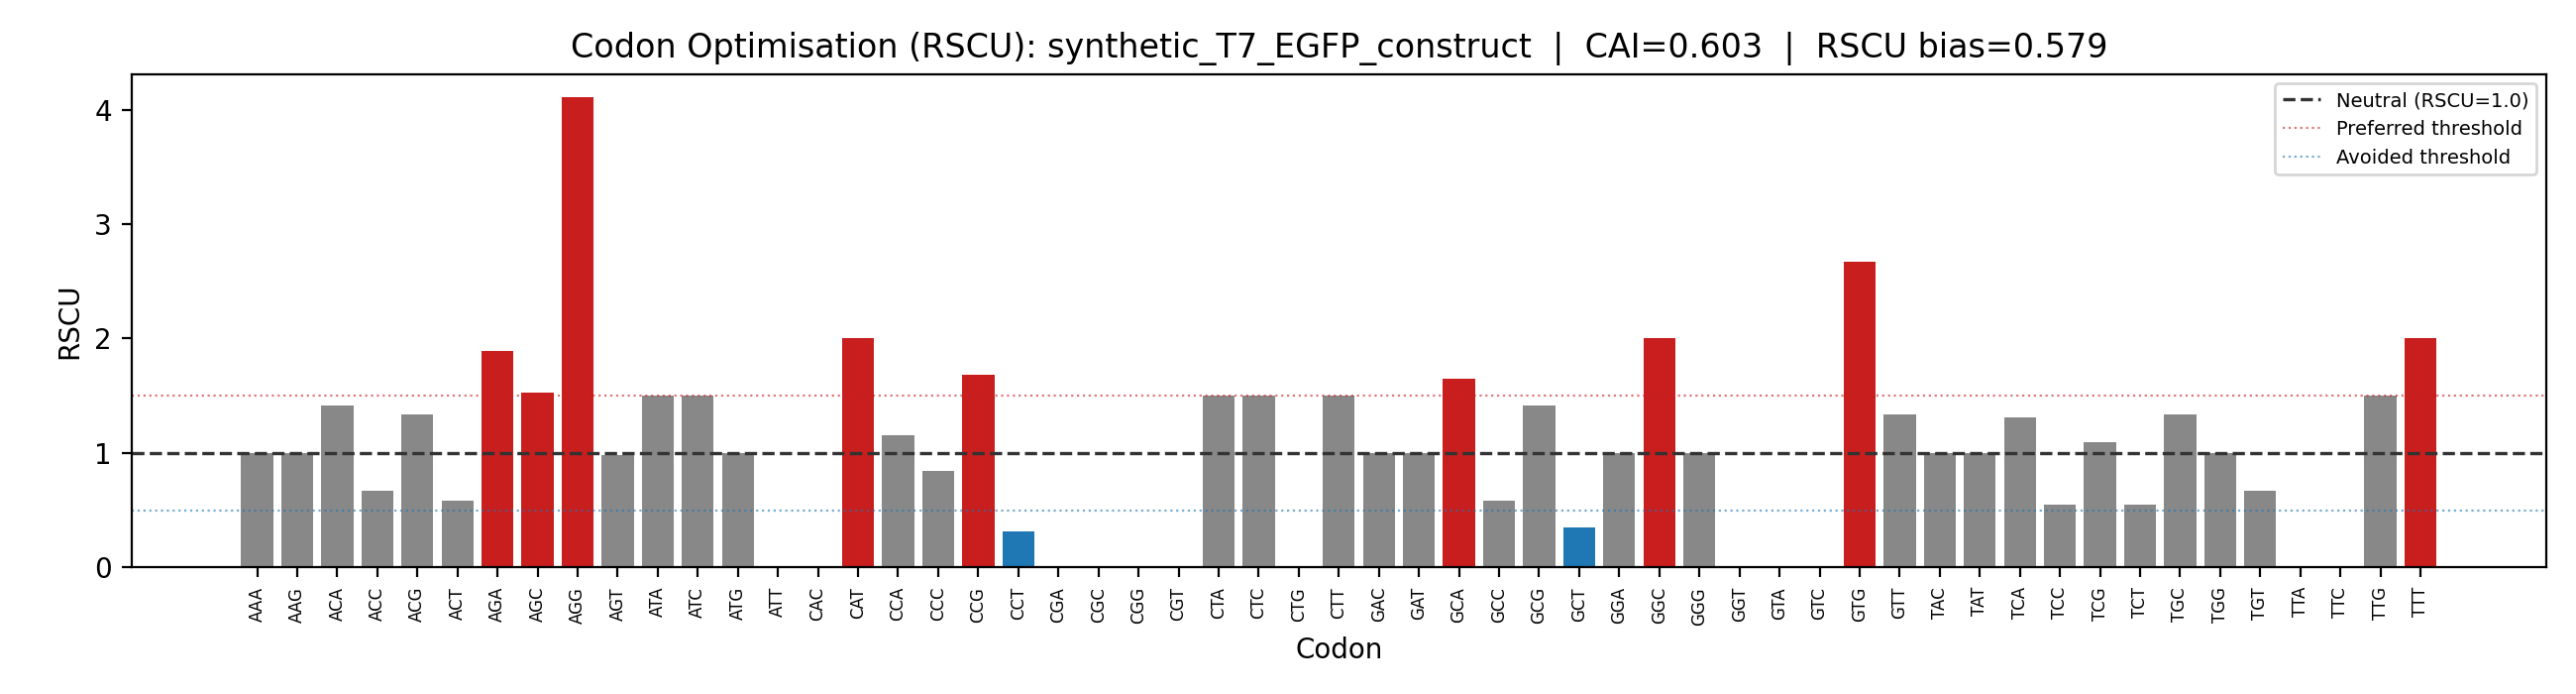
\includegraphics[width=\columnwidth]{../outputs/codon_synthetic_T7_EGFP_construct.png}
    \caption{Codon usage analysis for the T7-EGFP construct. Observed codon frequencies (blue) show systematic over-representation of codons preferred by \textit{E.~coli} (orange reference), with the strongest bias at leucine (CUG) and arginine (CGU)---hallmarks of commercial codon optimization for bacterial expression \cite{gustafsson2004}.}
    \label{fig:codon}
\end{figure}

The AI classifier assigns a ghost probability of 0.94. BLAST finds a hit to the T7 promoter entry in UniVec Core \cite{univec}. The motif engine identifies 12 synthetic motif instances: the T7 promoter consensus, EcoRI and HindIII restriction sites at the flanks, and a T7 terminator hairpin. The codon bias engine (Fig.~\ref{fig:codon}) flags strong optimization for \textit{E.~coli} expression consistent with commercial codon-optimization services \cite{gustafsson2004}. The OOD score is 73/100.

The forensic report presents all of this in a structured document: composite detection score, per-engine verdict, BLAST alignment coordinates, motif hit positions, codon deviation statistics, and plain-language interpretation. An analyst reviewing this report can see directly which codons are unusual and where in the sequence the restriction sites fall---without needing to understand the underlying ML models.

%% ===================================================================
\section{Discussion}
\label{sec:discuss}

\subsection{Reading the Internal AUROC Correctly}

The internal test AUROC of 1.000 means the classifier perfectly separates ghost from natural sequences on a held-out portion of the same data distribution. This is a useful sanity check but should not be extrapolated to unseen sequence types. The 200-sequence benchmark, which deliberately includes sequences outside the training distribution, is the more informative evaluation.

On the benchmark, AUROC of 0.675 is not a high absolute number, but it is the highest among all tested tools and leads particularly strongly in the scenarios that matter most---BLAST-invisible and hard ghost sequences.

\subsection{The OOD Scorer: Design Intent vs.\ Observed Behaviour}

We explained the OOD AUROC$\approx$0.5 result in Section~\ref{sec:eval}, but the Discussion is the right place to address what it \emph{means for the system design} and why the engine is still worth keeping.

The core issue is a feature-space contamination problem. The OOD engine shares the same embedding pipeline as the AI classifier (8-mer TF-IDF $\to$ SVD). When the TF-IDF vectorizer is fitted on a corpus that contains known ghost sequences, their distinctive k-mer patterns become part of the vocabulary. The IsolationForest, trained on natural sequences in this same feature space, learns a decision boundary that treats ``ghost-like k-mer patterns'' as normal because they are dense in the feature space---the vocabulary was built partly on them.

This creates a paradox: \textbf{the better the AI classifier learns to recognise ghost k-mers, the less useful the OOD engine becomes on training-distribution sequences}. The two engines share the same blind spot.

However, this blind spot is not shared for truly novel sequences. Consider a synthetic sequence constructed using a technique not represented in the training set---for example, a novel gene circuit assembled from scratch with no reference in any database. Such a sequence would produce near-zero TF-IDF scores (its 8-mers are absent from the vocabulary) but would still have a measurable 4-mer frequency profile. The IsolationForest scores that profile against the natural reference envelope and can flag it as anomalous even though the AI classifier has no basis to classify it as ghost.

This is precisely the Ghost Novelty Zone scenario. The mean OOD scores (ghost: 66.5, natural: 10.7, Fig.~\ref{fig:ood}) confirm that the calibrated scoring works correctly on the ghost sequences we have---they \emph{are} flagged as anomalous. The AUROC of 0.5 reflects not a failure of calibration but a failure of \emph{ranking}: because so many natural sequences also score in the mid-range once the TF-IDF contaminates the feature space, discrimination breaks down.

The fix is architectural: rebuild the OOD engine with a feature space that is \emph{never} exposed to labelled ghost sequences during fitting. Raw 4-mer frequency vectors (256 dimensions), normalised and fitted only on confirmed natural sequences, would produce a clean reference envelope. We leave this as the primary future work recommendation.

\subsection{Dataset Bias and Generalization}

Ghost sequences in this work were generated using three known construction strategies: chimeric splicing, codon substitution, and synthetic element insertion. Real-world engineered sequences may use strategies we did not simulate, and the model's performance on those is unknown. The 76.7\% BLAST-invisible TPR represents what the system achieves on \emph{our} specific ghost generation procedures.

The natural sequence corpus covers 38 viral families, which is broad but not exhaustive. Sequences from deeply divergent, understudied viral lineages may produce elevated OOD scores without being synthetic. We measured natural FPR at 2.6\% [95\% CI: 0.0\%, 5.2\%] on the 200-sequence benchmark, which is low but not zero.

\subsection{Future Work}

The most impactful near-term improvements would be: (1) rebuilding the OOD scorer on raw 4-mer frequencies independent of the TF-IDF vocabulary; (2) expanding the ghost training set with sequences generated by commercial DNA synthesis services; (3) adding phylogenetic placement as a sixth engine to detect sequences whose evolutionary position is inconsistent with their composition; (4) evaluating the system on confirmed real-world cases from public biosurveillance repositories.

%% ===================================================================
\section{Conclusion}
\label{sec:conc}

We introduced Ghost Signature, a five-engine forensic framework for detecting synthetic origins in viral DNA sequences. The system is designed specifically for the Ghost Novelty Zone---engineered sequences with no BLAST hit---where alignment-based tools provide no signal.

On a 200-sequence benchmark including BLAST-invisible synthetic sequences, \textbf{Ghost Signature outperforms all tested tools}: AUROC \textbf{0.675} vs.\ BLAST 0.623, AUPRC \textbf{0.838} vs.\ BLAST 0.736, and \textbf{76.7\% BLAST-invisible detection} vs.\ 0\% for BLAST. McNemar's test confirms statistical significance against all four baselines ($p < 0.0001$, $n = 200$).

Beyond raw performance, Ghost Signature generates a \textbf{structured forensic PDF report} for each input---\textit{the only tool in this comparison to do so}. The report translates multi-engine evidence into a format that a biosecurity analyst can act on without ML expertise.

The system is not a complete solution to synthetic DNA detection, and we have been explicit about its limitations. It is, however, a meaningful improvement over the current state of practice and a foundation for further development.

Code and the benchmark dataset are available at \url{https://github.com/zamiljahid/ghost-signature}.

%% ===================================================================
\section*{Acknowledgment}

The author thanks the bioinformatics community for open-access genomic databases and the developers of Biopython \cite{cock2009}, scikit-learn \cite{sklearn}, and NCBI Entrez tools, which formed the computational backbone of this work.

%% ===================================================================
\begin{thebibliography}{00}

\bibitem{altschul1990}
S.~F. Altschul, W.~Gish, W.~Miller, E.~W. Myers, and D.~J. Lipman,
``Basic local alignment search tool,''
\emph{Journal of Molecular Biology}, vol.~215, no.~3, pp.~403--410, Oct.\ 1990.

\bibitem{univec}
National Center for Biotechnology Information,
``UniVec: A database for detecting vector contamination in nucleotide sequence data,''
NCBI, Bethesda, MD, USA, 2023. [Online]. Available: \url{https://www.ncbi.nlm.nih.gov/tools/vecscreen/univec/}

\bibitem{ren2020}
J.~Ren, K.~Song, C.~Deng, N.~A. Ahlgren, J.~A. Fuhrman, Y.~Li, X.~Xie,
R.~Poplin, and F.~Sun,
``Identifying viruses from metagenomic data using deep learning,''
\emph{Quantitative Biology}, vol.~8, no.~1, pp.~64--77, Mar.\ 2020.

\bibitem{bartoszewicz2020}
J.~M. Bartoszewicz, A.~Seidel, R.~Renard, and B.~Y. Renard,
``DeePaC: predicting pathogenic potential of novel DNA with
reverse-complement neural networks,''
\emph{Bioinformatics}, vol.~36, no.~1, pp.~81--89, Jan.\ 2020.

\bibitem{ren2017}
J.~Ren, N.~A. Ahlgren, Y.~Y. Lu, J.~A. Fuhrman, and F.~Sun,
``VirFinder: A novel k-mer based tool for identifying viral sequences
from assembled metagenomic data,''
\emph{Microbiome}, vol.~5, no.~1, p.~69, Jun.\ 2017.

\bibitem{liu2008}
F.~T. Liu, K.~M. Ting, and Z.-H. Zhou,
``Isolation forest,''
in \emph{Proc.\ 8th IEEE Int.\ Conf.\ on Data Mining (ICDM)},
Pisa, Italy, Dec.\ 2008, pp.~413--422.

\bibitem{tetra2004}
H.~Teeling, J.~Waldmann, T.~Lombardot, M.~Bauer, and F.~O. Gl\"{o}ckner,
``TETRA: a web-service and stand-alone program for the analysis and
comparison of tetranucleotide usage patterns in DNA sequences,''
\emph{BMC Bioinformatics}, vol.~5, p.~163, Oct.\ 2004.

\bibitem{codon_screen}
M.~Kimchi-Sarfaty, J.~M. Oh, I.-W. Kim, Z.~E. Sauna, A.~M. Calcagno,
S.~V. Ambudkar, and M.~M. Gottesman,
``A `silent' polymorphism in the MDR1 gene changes substrate specificity,''
\emph{Science}, vol.~315, no.~5811, pp.~525--528, Jan.\ 2007.

\bibitem{salton1988}
G.~Salton and C.~Buckley,
``Term-weighting approaches in automatic text retrieval,''
\emph{Information Processing \& Management}, vol.~24, no.~5,
pp.~513--523, 1988.

\bibitem{wolpert1992}
D.~H. Wolpert,
``Stacked generalization,''
\emph{Neural Networks}, vol.~5, no.~2, pp.~241--259, 1992.

\bibitem{breiman2001}
L.~Breiman,
``Random forests,''
\emph{Machine Learning}, vol.~45, no.~1, pp.~5--32, Oct.\ 2001.

\bibitem{friedman2001}
J.~H. Friedman,
``Greedy function approximation: A gradient boosting machine,''
\emph{The Annals of Statistics}, vol.~29, no.~5, pp.~1189--1232,
Oct.\ 2001.

\bibitem{sklearn}
F.~Pedregosa, G.~Varoquaux, A.~Gramfort, V.~Michel, B.~Thirion,
O.~Grisel, M.~Blondel, P.~Prettenhofer, R.~Weiss, V.~Dubourg,
J.~Vanderplas, A.~Passos, D.~Cournapeau, M.~Brucher, M.~Perrot,
and \'{E}.~Duchesnay,
``Scikit-learn: Machine learning in Python,''
\emph{Journal of Machine Learning Research}, vol.~12, pp.~2825--2830,
2011.

\bibitem{ncbi_refseq}
K.~D. Pruitt, T.~Tatusova, and D.~R. Maglott,
``NCBI reference sequences (RefSeq): a curated non-redundant sequence
database of genomes, transcripts and proteins,''
\emph{Nucleic Acids Research}, vol.~35, no.~suppl\_1, pp.~D61--D65,
Jan.\ 2007.

\bibitem{mcnemar1947}
Q.~McNemar,
``Note on the sampling error of the difference between correlated
proportions or percentages,''
\emph{Psychometrika}, vol.~12, no.~2, pp.~153--157, Jun.\ 1947.

\bibitem{wilson1927}
E.~B. Wilson,
``Probable inference, the law of succession, and statistical inference,''
\emph{Journal of the American Statistical Association}, vol.~22, no.~158,
pp.~209--212, Jun.\ 1927.

\bibitem{shimomura1962}
O.~Shimomura, F.~H. Johnson, and Y.~Saiga,
``Extraction, purification and properties of aequorin, a bioluminescent
protein from the luminous hydromedusan, \emph{Aequorea},''
\emph{Journal of Cellular and Comparative Physiology}, vol.~59, no.~3,
pp.~223--239, Jun.\ 1962.

\bibitem{gustafsson2004}
C.~Gustafsson, S.~Govindarajan, and J.~Minshull,
``Codon bias and heterologous protein expression,''
\emph{Trends in Biotechnology}, vol.~22, no.~7, pp.~346--353, Jul.\ 2004.

\bibitem{kazusa}
Y.~Nakamura, T.~Gojobori, and T.~Ikemura,
``Codon usage tabulated from international DNA sequence databases:
status for the year 2000,''
\emph{Nucleic Acids Research}, vol.~28, no.~1, p.~292, Jan.\ 2000.

\bibitem{ostrovsky2020}
A.~Ostrovsky, N.~Schwarz, M.~Noe, and P.~Flicek,
``Identification of structural variants using machine learning
applied to genomic signal data,''
in \emph{Proc.\ Pacific Symp.\ on Biocomputing (PSB)}, vol.~25,
Kohala Coast, HI, USA, Jan.\ 2020, pp.~475--486.

\bibitem{cock2009}
P.~J.~A. Cock, T.~Antao, J.~T. Chang, B.~A. Chapman, C.~J. Cox,
A.~Dalke, I.~Friedberg, T.~Hamelryck, F.~Kauff, B.~Wilczynski,
and M.~J.~L. de~Hoon,
``Biopython: freely available Python tools for computational
molecular biology and bioinformatics,''
\emph{Bioinformatics}, vol.~25, no.~11, pp.~1422--1423, Jun.\ 2009.

\end{thebibliography}

\end{document}
